% Fig 2.3 — Dense vs Sparse retrieval, side-by-side
% Two-column comparison showing each retriever's pipeline for the same query.

\documentclass[border=4pt]{standalone}
\usepackage{tikz}
\usetikzlibrary{positioning, arrows.meta, fit, backgrounds}

\begin{document}
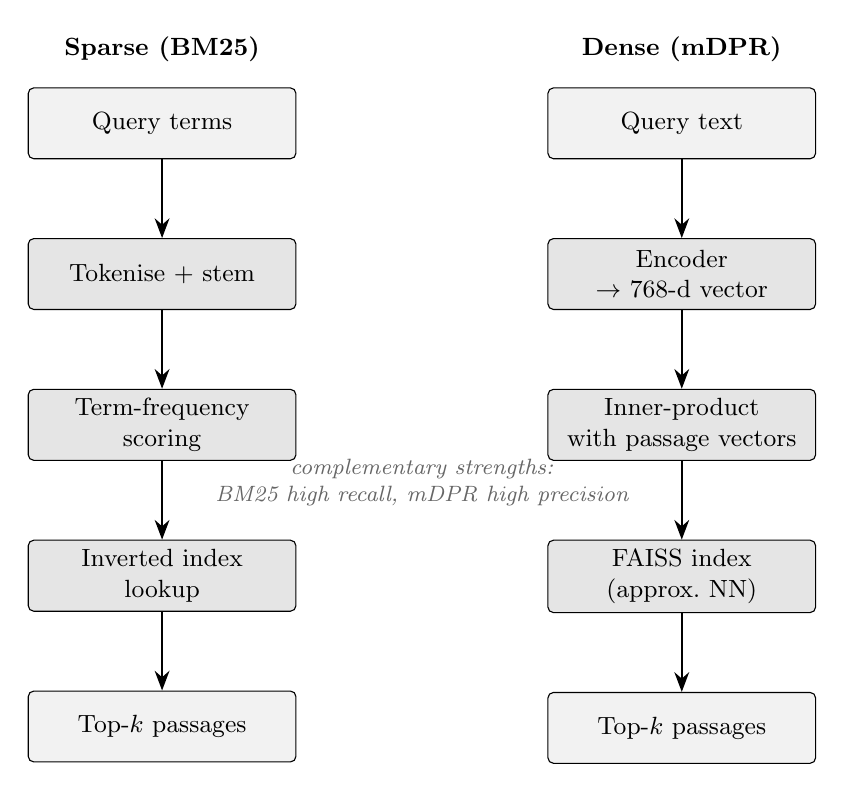
\begin{tikzpicture}[
    >=Stealth,
    box/.style={rectangle, draw, rounded corners=2pt,
                minimum width=34mm, minimum height=9mm,
                align=center, font=\small},
    header/.style={font=\bfseries\small},
    arrow/.style={-{Stealth[length=2.5mm]}, thick},
    note/.style={font=\footnotesize\itshape, color=black!60}
]
  % --- Sparse column (left) ---
  \node[header] (sparseH) at (-26mm, 5mm) {Sparse (BM25)};
  \node[box, fill=black!5, below=2mm of sparseH] (sq) {Query terms};
  \node[box, fill=black!10, below=of sq] (stok) {Tokenise + stem};
  \node[box, fill=black!10, below=of stok] (sscore) {Term-frequency\\scoring};
  \node[box, fill=black!10, below=of sscore] (sidx) {Inverted index\\lookup};
  \node[box, fill=black!5, below=of sidx] (sout) {Top-$k$ passages};

  \draw[arrow] (sq) -- (stok);
  \draw[arrow] (stok) -- (sscore);
  \draw[arrow] (sscore) -- (sidx);
  \draw[arrow] (sidx) -- (sout);

  % --- Dense column (right) ---
  \node[header] (denseH) at (40mm, 5mm) {Dense (mDPR)};
  \node[box, fill=black!5, below=2mm of denseH] (dq) {Query text};
  \node[box, fill=black!10, below=of dq] (denc) {Encoder \\$\rightarrow$ 768-d vector};
  \node[box, fill=black!10, below=of denc] (dscore) {Inner-product\\with passage vectors};
  \node[box, fill=black!10, below=of dscore] (didx) {FAISS index\\(approx.\ NN)};
  \node[box, fill=black!5, below=of didx] (dout) {Top-$k$ passages};

  \draw[arrow] (dq) -- (denc);
  \draw[arrow] (denc) -- (dscore);
  \draw[arrow] (dscore) -- (didx);
  \draw[arrow] (didx) -- (dout);

  % Centre note
  \node[note, align=center] at (7mm, -50mm)
    {complementary strengths:\\BM25 high recall, mDPR high precision};

\end{tikzpicture}
\end{document}
